% Atualizado para atender as normas ABNT por Mônica da Silva (04/11/2021)

% --- -----------------------------------------------------------------
% --- Elementos usados na Capa e na Folha de Rosto.
% --- EXPRESSÔES ENTRE <> DEVERÂO SER COMPLETADAS COM A INFORMAÇÂO ESPECÍFICA DO TRABALHO
% --- E OS SÌMBOLOS <> DEVEM SER RETIRADOS 
% --- -----------------------------------------------------------------
\autor{André Fernandes Gonçalves} % deve ser escrito em maiúsculo

\titulo{Classificação de Alagamento em Vias com Tráfego na Cidade do Rio de Janeiro através de Visão Computacional}

\instituicao{UNIVERSIDADE FEDERAL FLUMINENSE}

\orientador{Aura Conci}

%\coorientador{<NOME DO COORIENTADOR>} % se nao existir co-orientador apague essa linha

\local{NITER\'{O}I}

\data{2025} % ano da defesa

\comentario{Dissertação de Mestrado apresentada ao Programa de P\'{o}s-Gradua\c{c}\~{a}o em Computa\c{c}\~{a}o da \mbox{Universidade} Federal Fluminense como requisito parcial para a obten\c{c}\~{a}o do Grau de \mbox{Mestre em Computa\c{c}\~{a}o}. \'{A}rea de concentra\c{c}\~{a}o: \mbox{Computa\c{c}\~{a}o}} %preencha com a sua área de concentração


% --- -----------------------------------------------------------------
% --- Capa. (Capa externa, aquela com as letrinhas douradas)(Obrigatório)
% --- ----------------------------------------------------------------
\capa

% --- -----------------------------------------------------------------
% --- Folha de rosto. (Obrigatório)
% --- ----------------------------------------------------------------
\folhaderosto

% --- -----------------------------------------------------------------
% --- Ficha catalográfica obrigatória na versão final. (Obrigatório)
% --- ----------------------------------------------------------------

\begin{figure}[!ht]
   \centering
   %
\includegraphics[width=1\linewidth]{capitulos/figuras/ficha_catalografica.png}
   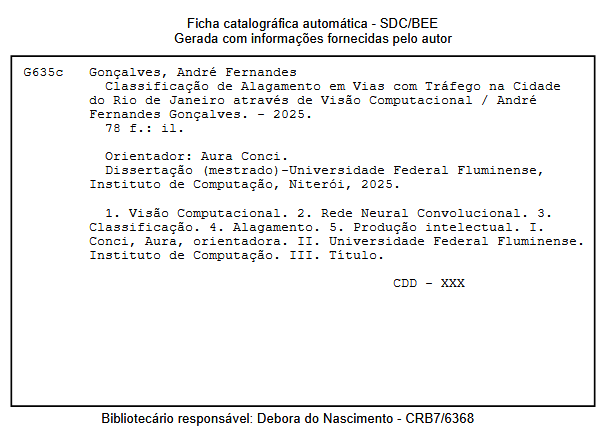
\includegraphics[width=1\linewidth]{images/fichacatalografica.png}
   %\caption{Local da ficha catalográfica}
\end{figure}

\cleardoublepage


\pagestyle{ruledheader}
\setcounter{page}{1}
\pagenumbering{roman}

% --- -----------------------------------------------------------------
% --- Termo de aprovação. (Obrigatório)
% --- ----------------------------------------------------------------
\cleardoublepage
\thispagestyle{empty}

\vspace{-60mm}

\begin{center}
   {\large ANDRÉ FERNANDES GONÇALVES}\\
   \vspace{7mm}

   \uppercase{Classificação de Alagamento em Vias com Tráfego na Cidade do Rio de Janeiro através de Visão Computacional}\\
  \vspace{10mm}
\end{center}

\noindent
\begin{flushright}
\begin{minipage}[t]{8cm}

Dissertação de Mestrado apresentada ao Programa de P\'{o}s-Gradua\c{c}\~{a}o em Computa\c{c}\~{a}o da Universidade Federal Fluminense como requisito parcial para a obten\c{c}\~{a}o do \mbox{Grau} de Mestre em Computa\c{c}\~{a}o. \'{A}rea de concentra\c{c}\~{a}o: \mbox{Computa\c{c}\~{a}o} %preencha com a sua área de concentração

\end{minipage}
\end{flushright}
\vspace{1.0 cm}
\noindent
Aprovada em MARÇO de 2025. \\
\begin{flushright}
 % \parbox{11cm}
  {
  \begin{center}
  BANCA EXAMINADORA \\
  \vspace{6mm}
  \rule{11cm}{.1mm} \\
    Prof. Aura Conci - Orientadora, UFF \\
    \vspace{6mm}
  \rule{11cm}{.1mm} \\
    Prof. Leandro Augusto Frata Fernandes, UFF\\
    \vspace{6mm}
  \rule{11cm}{.1mm} \\
    Prof. Flávia Cristina Bernardini, UFF\\
  \vspace{4mm}
  \rule{11cm}{.1mm} \\
    Prof. Aristófanes Corrêa Silva, UFMA\\
    \vspace{6mm}
  \rule{11cm}{.1mm} \\
    Prof. Raul Queiroz Feitosa, PUC\\
  \vspace{6mm}
  \end{center}
  }
\end{flushright}
\begin{center}
  \vspace{4mm}
  Niter\'{o}i \\
  %\vspace{6mm}
  2025

\end{center}

% --- -----------------------------------------------------------------
% --- Dedicatoria.(Opcional)
% --- -----------------------------------------------------------------
\cleardoublepage
\thispagestyle{empty}
\vspace*{200mm}

\begin{flushright}
{\em 
    Aos meus pais, que me apoiaram ao longo da minha jornada.
}
\end{flushright}
\newpage


% --- -----------------------------------------------------------------
% --- Agradecimentos.(Opcional)
% --- -----------------------------------------------------------------
\pretextualchapter{Agradecimentos}
\hspace{5mm}
A minha orientadora, Aura Conci, que me ajudou em todo o caminho e sempre confiou em mim.

A UFF e a CAPES, pela bolsa que me ajudou durante meus estudos do mestrado.

A Luis Rezende e Otávio Flaeschen pela ajuda na criação do conjunto de dados.

Ao Centro de Operações do Rio pelo acesso as câmeras da cidade do Rio de Janeiro.

% --- -----------------------------------------------------------------
% --- Resumo em português.(Obrigatório)
% --- -----------------------------------------------------------------
\begin{resumo}

%Elemento obrigatório, constituído de uma sequência de frases concisas e objetivas e não de uma simples enumeração de tópicos, não ultrapassando 500 palavras ABNT NBR 6028:2003.

Este trabalho teve como objetivo desenvolver uma abordagem inicial para a classificação automática de alagamentos da cidade do Rio de Janeiro.
Para isso, primeiramente foi criado um conjunto de dados original, o \acrfull{rfd}, composto de 4620 imagens separadas em 78\% para treino e 22\% para validação.
Este conjunto de dados foi montado com imagens de câmeras de ruas da cidade do Rio ao longo de diferentes meses, em diferentes horas do dia e com diversos níveis de alagamento.
Após o conjunto de dados ser devidamente analisado e montado de forma equilibrada, cinco arquiteturas de redes neurais foram utilizadas nesse conjunto de dados. 
Essas arquiteturas foram escolhidas de acordo com trabalhos da literatura com temática relacionada ao problema abordado.
Após o treinamento das arquiteturas \acrshort{vgg}-19, \textit{Inception}, \textit{DenseNet}, \textit{MobileNetV2}, e \textit{Visual Transformer} para o problema de classificação de imagem, 
o \textit{Visual Transformer} obteve melhor resultado. Este modelo, o \textit{Visual Transformer}, foi analisado com diferentes níveis de iluminação e três diferentes otimizadores.
Também foi investigado se o aumento na quantidade de imagens de treino traria ganhos compensadores. 
O desempenho dos resultados foi comparado com outros dois conjuntos de dados.
Considerando todos os experimentos feitos, o \textit{Visual Transformer} foi o melhor modelo com acurácia de 82,6\% no conjunto de dados original.
O código usado para treino e avaliação dos modelos estão disponíveis \href{https://github.com/afego/computervision}{neste repositório de GitHub}: https://github.com/afego/computervision.
O conjunto de dados original está disponível em \href{https://doi.org/10.5281/zenodo.15670835}{10.5281/zenodo.15670835}.

{\hspace{-8mm} \bf{Palavras-chave}}: Visão Computacional, Rede Neural Convolucional, \textit{Visual Transformer}, Classificação, Alagamento.

\end{resumo}

% --- -----------------------------------------------------------------
% --- Resumo em língua estrangeira.(Obrigatório)
% --- -----------------------------------------------------------------
\begin{abstract}

%Elemento obrigatório, em língua estrangeira, com as mesmas características do resumo em língua vernácula (ABNT, 2005).
%O resumo deve ser redigido na terceira pessoa do singular, com verbo na voz ativa, não ultrapassando uma página ou 500 palavras, segundo a ABNT NBR 6028). Evitando-se ouso de parágrafos no meio do resumo, assim como fórmulas, equações e símbolos. Iniciar o resumo situando o trabalho no contexto geral, apresentar os objetivos, descrever a metodologia utilizada, relatar a contribuição própria, comentar os resultados obtidos e finalmente apresentaras conclusões mais importantes do trabalho.

This work aimed to develop an initial approach for the automatic classification of floods in the city of Rio de Janeiro.
To this end, this work first created an original dataset composed of 4620 images separated into 78\% for training and 22\% for validation.
This dataset was assembled with images from street cameras in the city of Rio over different months, at different times of the day and at various flood levels.
After the dataset was properly analyzed and assembled in a balanced way, five neural network architectures were evaluated on this dataset.
These architectures were chosen according to works in the literature with a theme related to the problem addressed.
After training the \acrshort{vgg}-19, \textit{Inception}, \textit{DenseNet}, \textit{MobileNetV2}, and \textit{Visual Transformer} architectures for the image classification problem,
the \textit{Visual Transformer} obtained the best result. The \textit{Visual Transformer} was then also analyzed with different lighting levels and three different optimizers.
It was also investigated whether increasing the number of training images would bring compensating gains.
The performance of the results was compared with two other datasets.
Considering all experiments done, the \textit{Visual Transformer} was the best model with an accuracy of 82.6\% on the original dataset.
The code used for training and evaluating the models is available \href{https://github.com/afego/computervision}{in this GitHub repository}: https://github.com/afego/computervision.
The novel dataset from this research is available at \href{https://doi.org/10.5281/zenodo.15670835}{10.5281/zenodo.15670835}.

{\hspace{-8mm} \bf{Keywords}}: Computer Vision, Convolutional Neural Network, \textit{Visual Transformer}, Classification, Flooding

\end{abstract}

% --- -----------------------------------------------------------------
% --- Lista de figuras.(Opcional)
% --- -----------------------------------------------------------------
%\cleardoublepage
\listoffigures



% --- -----------------------------------------------------------------
% --- Lista de tabelas.(Opcional)
% --- -----------------------------------------------------------------
\cleardoublepage
%\label{pag:last_page_introduction}
\listoftables
\cleardoublepage

% --- -----------------------------------------------------------------
% --- Lista de abreviatura.(Opcional)
%Elemento opcional, que consiste na relação alfabética das abreviaturas e siglas utilizadas no texto, seguidas das %palavras ou expressões correspondentes grafadas por extenso. Recomenda-se a elaboração de lista própria para cada %tipo (ABNT, 2005).
% --- ----------------------------------------------------------------

\cleardoublepage
\printglossary[type=\acronymtype,title={Lista de Abreviaturas e Siglas}]
\cleardoublepage


% --- -----------------------------------------------------------------
% --- Sumario.(Obrigatório)
% --- -----------------------------------------------------------------

\pagestyle{ruledheader}
\tableofcontents
\pagebreak